\section{Experiment design}

\subsection{Hardware and software}

We used a single Google Pixel 6a (codename \textit{bluejay}) to install and evaluate studied Android distributions. This model was chosen due to its broad compatibility with alternative operating systems. The full measurement setup is shown in Fig.~\ref{fig-devices}.  All tested builds base on Android 16 and were obtained in December 2025:
\begin{itemize}
	\item Stock Android: \texttt{BP4A.251205.006}
	\item LineageOS: \texttt{lineage-23.0-20251206} (\texttt{BP2A.250805.005})
	\item LineageOS for microG: \texttt{lineage-23.0-20251203-microG}
	(\texttt{BP2A.250805.005})
	\item GrapheneOS: \texttt{2025121200} (\texttt{BP4A.251205.006})
	\item iod\'eOS: \texttt{7.0-20251129-bluejay} (\texttt{BP2A.250805.005})
\end{itemize}

\begin{figure}
	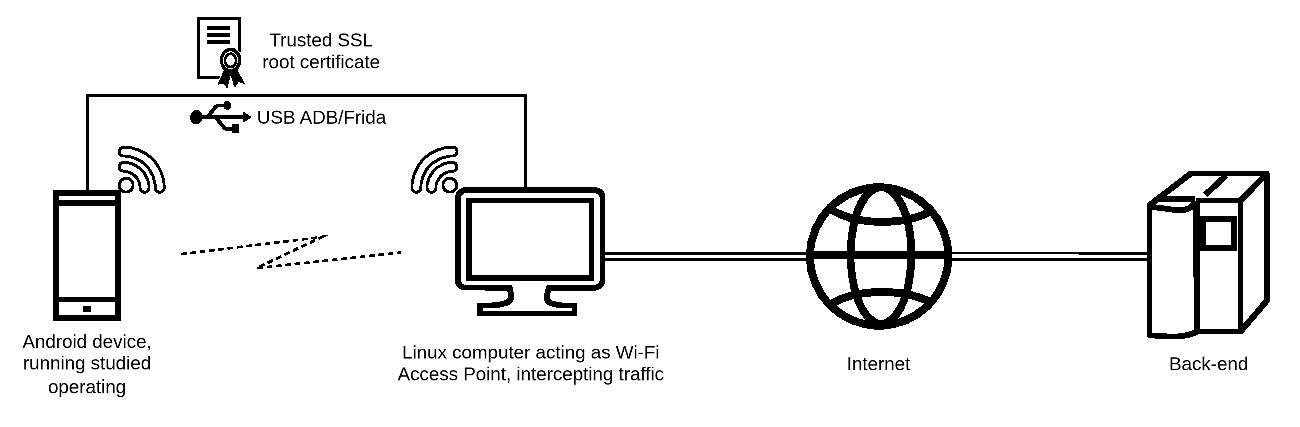
\includegraphics[width=\textwidth]{images/devices.eps}
	\caption{Measurement setup. Android device running studied operating systems is configured to access Internet using Wi-Fi. Access point is hosted on a Linux computer, running traffic interception and capturing software. Custom system certificate is installed on the phone using root access. USB connection is used for ADB/Frida communication.} \label{fig-devices}
\end{figure}

\subsection{Measurement scenarios}
To enable consistent, comparable measurements across Android distributions, four setup scenarios were defined. Each scenario specifies the Google account state, consent and permission posture, and which Google components are present. Not all scenarios apply to every operating system due to their characteristics. Scenarios were adapted to each system's capabilities: on GrapheneOS, sandboxed Google Play Services were installed immediately after setup; on systems with microG, the component was enabled during initial setup when prompted, or activated manually immediately afterward. As a general principle, any required configuration step not available during initial setup was performed as soon as possible thereafter.

\paragraph{Scenario A: Default Setup with Google Account.}
The device is configured to reflect a typical user path. Google account sign-in is performed during setup (or immediately after) and default recommendations are accepted (including prompted permissions).

\paragraph{Scenario A2: Minimal Setup with Google Account.}
This scenario extends \textit{Scenario A} by adjusting settings towards privacy while retaining Google account functionality. During and after initial setup, all optional consents and permissions are declined. System and account settings are adjusted to maximize user privacy. This scenario is not applicable to systems using microG or GrapheneOS, as these distributions are already designed to minimize privacy risks and do not implement or prompt users for privacy-threatening features characteristic of the factory system.

\paragraph{Scenario B: Minimal Setup without Google Account.}
The device is configured with maximum privacy in mind, avoiding Google account sign-in entirely. During initial setup, only strictly required prompts are accepted and optional data-sharing is declined. System settings are  adjusted to maximize user privacy. Google components or their functional replacements remain present and enabled to preserve baseline device functionality and app compatibility, but operate without account.

\paragraph{Scenario C: Extremely Minimal Setup without Google Components.}
This scenario applies only to distributions that do not bundle or enable Google services by default. It is not applicable to the official factory system, which enables Google components by default. If microG is preinstalled, it remains disabled.

\subsection{Measurement tasks}
We performed the following measurement tasks sequentially for each scenario. Network traffic was captured using Wireshark for basic analysis.

\paragraph{Task 0: Initial setup.}
Configure the device according to the target scenario, connect to Wi-Fi, complete account sign-ins and install components as specified. Network traffic capture begins with the device's first Internet connection and continues until 10 minutes after setup completion.

\paragraph{Task 1: System idle.}
Ensure the system and apps are up to date and that no update-related background jobs are running. Reboot the device to begin capture, then keep it connected to the monitored network for at least 30 minutes. During this period, unlock the device three times and scroll through the app list. Do not open any apps.

\paragraph{Task 2: Basic apps interactions.}
Open preinstalled apps and perform simple actions that should not require an Internet connection
\begin{itemize}
	\item Settings: disable haptic feedback; toggle dark mode; check per-app battery usage
	\item Clock: set an alarm
	\item Files: create a folder
	\item Contacts: create a local (on-device) contact
\end{itemize}

Beyond direct task comparisons, additional packets of interest were examined to compare data transmission practices across different system configurations and to characterize what data is sent and how. This analysis required TLS decryption via the intercepting proxy and, in some cases, runtime certificate unpinning with Frida using scripts from HTTP Toolkit.\footnote{\url{https://github.com/httptoolkit/frida-interception-and-unpinning}} Although Frida-based unpinning failed in most attempts, it was useful in a small number of cases. When useful, we used publicly available Protocol Buffer definitions from microG's source code to decode payloads.

To complement network-level observations, Google Takeout\footnote{\url{https://takeout.google.com/}} was used to inspect server-side data associated with the test Google account after running scenarios involving Google services (Stock Android, GrapheneOS with sandboxed Google Play Services, and microG-based distributions).